\scanpage{51}
\mspage{\handwritten{19}}
% archive sheet number: 50

\deleted{open (EGA IV 2.4.9), it \deleted{not} suffices to prove that ther\deleted{\unsure{o|h}}\inserted{e} exists such an extension $k'$ and a point $x'$ of $H'=H\otimes_k k'$ above $x$, such that $H'-G'$ is a neighborhood of $x'$. Now \deleted{one}\handwritten{it} will suffice to take \deleted{$k$} $k'=k(x)$, so that $G'$ admits a point $x'$ rational over $k'$ above $x$. Then the open subset in $H'$ which is the translate of $G'$ by $x'$ contains $x'$ and is contained in $H'-G'$\handwritten{,}\deleted{\unsure{which}} which is therefore a neighborhood of $x'$, which completes the proof of 11.11.}

\uline{Remark} 11.11.\deleted{\unsure{3|1}}\handwritten{1}. \deleted{Mister} M. Raynaud points out to us that one can generali-\linebreak ze 11.11 to the case of a quasi-compact and quasi-s\deleted{p}\handwritten{e}\deleted{\unsure{é|e}}\handwritten{p}arated group scheme $G$ over a regular scheme\inserted{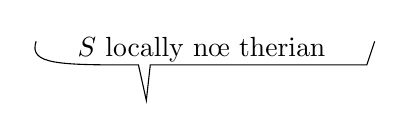
\begin{tikzpicture}[x=1cm,y=1cm,baseline=(n.base)]\node (n) at (0,0) {$S$ locally n\oe{} therian};\draw (-2.1,.1) .. controls (-2.2,-.2) and (-1.8,-.2) .. (-.8,-.2)--(-.7,-.65)--(-.65,-.2)--(2.1,-.2)--(2.2,.1);\end{tikzpicture}} of dimension $\handwritten{\leqslant}1$, assuming moreover $G$ \uline{flat} over $S$. 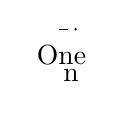
\begin{tikzpicture}[x=1cm,y=1cm,baseline=(n.base)]\node (n) at (0,0) {One};\node at (.12,-.26) {\handwritten{n}};\draw (-.03,.33)--(.08,.33);\fill (.18,.33) circle (.018);\end{tikzpicture} then has equivalence of the following conditions:

(i) $G$ is affine over $S$.

(ii) $G$ is quasi-affine over $S$.

(iii) \unsure{G|O}ne can make $G$ act faithfully on a quasi-affine $S$-scheme.

(iv) One can make $G$ act faithfully on a quasi-coherent Module flat over $S$.

(v) (If $G$ is of finite type over $S$\inserted{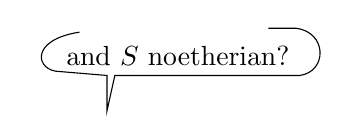
\begin{tikzpicture}[x=1cm,y=1cm,baseline=(n.base)]\node (n) at (0,0) {and $S$ noetherian\handwritten{?}};\draw (-1.25,.3) .. controls (-1.9,.2) and (-1.8,-.2) .. (-1.5,-.2)--(-.9,-.25)--(-.9,-.7)--(-.8,-.25)--(1.55,-.25) .. controls (1.9,-.2) and (1.9,.3) .. (1.5,.35)--(1.15,.35);\end{tikzpicture}}) $G$ is isomorphic to a closed subgroup of an $\text{\uline{Aut}}_V$, where $V$ is a locally free Module of finite type over $\handwritten{\unsure{\mathbb{S}|S}}$.

% Handwritten relocation arrow, from the lower remark towards the upper remark.
\margin{\figure{\handwritten{\begin{tikzpicture}[x=0.35cm,y=0.35cm]\draw (1,0) .. controls (0.1,-0.3) and (0.1,0.1) .. (0.1,0.7) -- (0.1,2) .. controls (0.1,2.7) and (0.4,2.8) .. (1,2.8);\draw (0.2,2.5) .. controls (-.6,3.5) and (-.7,6.2) .. (-.9,8.0);\draw[->] (-.92,8.15) .. controls (-.97,9.3) and (-1,10.5) .. (-.8,11) .. controls (-.4,12) and (0.5,12.4) .. (1.6,12.5);\end{tikzpicture}}}}
\deleted{\uline{Remark} 11.11.2. With the notation of the preceding proof, one sees easily (once one knows that $G$ is affine) that \unsure{G'|the} homomor-\linebreak phism $G\handwritten{\longrightarrow}G'=\underset{\handwritten{\longleftarrow}}{\lim}G_i$ is an isomorphism, which gives for $G$ a structure theorem\handwritten{,} which will be \deleted{taken up again}\inserted{proved} by another method in 11.1\deleted{\unsure{3}}\handwritten{5}.}
